\documentclass[a4paper]{report}

\usepackage{amsmath,amssymb,stmaryrd,latexsym}
\usepackage{titlepic}
\usepackage{syntax}
\usepackage{multicol}
\usepackage{alltt}
\usepackage{graphicx}   % Including Graphics
%\usepackage{verbatim} 
\usepackage{spverbatim}
\usepackage{alltt} 
\usepackage{xspace} 
\usepackage{listings} 
\usepackage{ifthen}
\usepackage{adjustbox}
\usepackage{xhfill}% http://ctan.org/pkg/xhfill
\usepackage{color}
\usepackage{fancybox}
\usepackage{fancyvrb}
\usepackage{fixltx2e}
\usepackage[multiple]{footmisc}
\usepackage{grammar-defns}  %% Generated by Obelisk
\usepackage{url}
\usepackage{bcprules}

\newsavebox{\FVerbBox}
\newenvironment{FVerbatim}
 {\VerbatimEnvironment
  \begin{center}
  \begin{lrbox}{\FVerbBox}
  \begin{BVerbatim}}
 {\end{BVerbatim}
  \end{lrbox}
  \fbox{\usebox{\FVerbBox}}
  \end{center}}

\newboolean{devel}
\setboolean{devel}{true}

\lstloadlanguages{C++,VHDL}
\lstset{frameround=tttt} 
\lstset{captionpos=t}
\lstset{breaklines=true}
\lstset{escapechar=@}
%\lstset{aboveskip=2\medskipamount}
%\lstset{belowskip=1.5\medskipamount}
%\lstset{abovecaptionskip=\medskipamount}
\lstdefinelanguage{Rfsm}{keywords={type,enum,record,function,return,fsm,model,in,out,inout,vars,states,trans,itrans,on,when,with,periodic,sporadic,value_changes,event,bool,input,output,shared,where,and},morecomment=[l]{--}}
\lstdefinelanguage{ctask}{language=C,morekeywords={task,wait_ev,wait_evs,notify_ev,in,out,inout}}
\lstdefinelanguage{systemc}{language=C++,morekeywords={SC_MODULE,SC_METHOD,SC_THREAD,sc_in,sc_out,sc_inout}}

%%% Better hyphenation:
%\sloppy
\setlength{\topmargin}{0pt}
\setlength{\oddsidemargin}{0pt}
\setlength{\textheight}{600pt}
\setlength{\textwidth}{448pt}

%\Newcommand{\docdate}{\today} %%%!!!!
\newcommand{\step}{\noindent\medskip$\blacktriangleright$\xspace}

\newcommand{\version}{2.0}

\newcommand{\ie}{\emph{i.e.}\xspace}
\newcommand{\txt}[1]{\hbox{#1}}
\newcommand{\emtxt}[1]{\hbox{\em{#1}}}
\newcommand{\bftxt}[1]{\hbox{\bf{#1}}}
\ifthenelse{\boolean{devel}}{\newcommand{\note}[1]{\marginpar{\tiny #1}}}{\newcommand{\note}[1]{}}
\newcommand{\todo}[1]{\note{TODO: #1}}
\newcommand{\tofix}[1]{\note{TOFIX: #1}}
\ifthenelse{\boolean{devel}}{\newcommand{\tbw}[1]{$\spadesuit$ {\bf To be written\ldots}\xspace}}{\newcommand{\tbw}[1]{}}
\ifthenelse{\boolean{devel}}{\newcommand{\tbc}[1]{$\spadesuit$ {\bf To be continued\ldots}\xspace}}{\newcommand{\tbc}[1]{}}

\newcommand{\rfsm}{RFSM\xspace}
\newcommand{\ocaml}{{\sc Objective Caml}\xspace}

\newcommand{\example}[1]{\fcolorbox{white}{lightgray}{#1}}
\newcommand{\ifname}[3]{$\mathtt{#1}_{\mathtt{#2}}\mathtt{#3}$}

%\newenvironment{example}{\medskip\noindent{\it Example :}\begin{alltt}}{\end{alltt}}

\title{RFSM Reference Manual - \version}

\author{J. S\'erot}

\titlepic{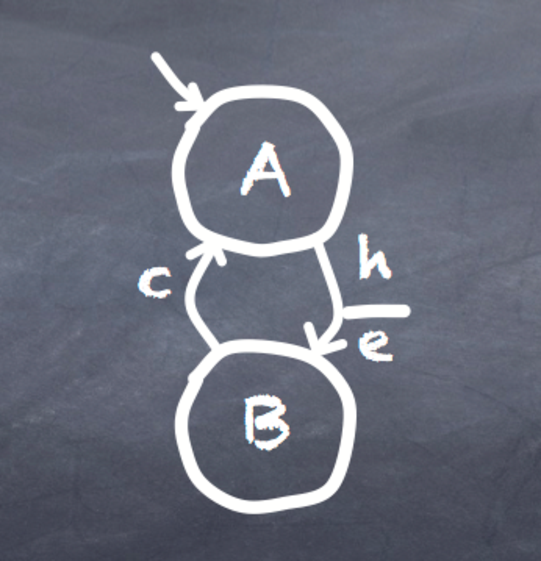
\includegraphics[width=0.5\textwidth]{../figs/rfsm-logo}}
\date{}

\begin{document}

\maketitle

%\tableofcontents

\chapter{ Formal syntax of RFSM programs}
\label{cha:bnf}

This appendix gives a BNF definition of the concrete syntax RFSM programs.
As stated in the introduction, this syntax is that of the so-called \emph{standard} RFSM language.
Variant languages will essentially differ in the definition of the
$\rfsmtypedecl*{}$,
$\rfsmtypeexpr*{}$,
$\rfsmexpr*{}$,
$\rfsmconstant*{}$,
and $\rfsmconst*{}$
syntactical categories.

\medskip
The meta-syntax is conventional. Keywords are written in \textbf{boldface}.  Non-terminals are
enclosed in angle brackets ({\tt <} \ldots {\tt >}).  Vertical bars ({\tt |}) indicate
alternatives.  Constructs enclosed in non-bold brackets ({\tt [} \ldots {\tt ]}) are optional.
The notation $E^*$ (resp $E^+$) means zero (resp one) or more repetitions of $E$, separated by spaces.
The notation $E^*_x$ (resp $E^+_x$) means zero (resp one) or more repetitions of $E$, separated by
symbol $x$. Terminals \verb|lid| and \verb|uid| respectively designate identifiers
starting with a lowercase and uppercase letter. 

\begin{rfsmgrammar}
\rfsmgramfunc{\rfsmprogram{}}& \rfsmgramdef & \rfsmgramstar{\rfsmtypedecl*{}} \\ & &
                                              \rfsmgramstar{\rfsmcstdecl*{}} \\ & &
                                              \rfsmgramstar{\rfsmfndecl*{}} \\ & &
                                              \rfsmgramstar{\rfsmfsmmodel*{}} \\ & &
                                              \rfsmgramstar{\rfsmfsmmodel*{}} \\ & &
                                              \rfsmgramstar{\rfsmglobal*{}} \\ & &
                                              \rfsmgramstar{\rfsmfsminst*{}}
                                              \rfsmEOF*{}
  \\& & \\

\rfsmgramfunc{\rfsmtypedecl{}}& \rfsmgramdef & \rfsmTYPE*{} \rfsmLID*{}
                                               \rfsmEQUAL*{} \rfsmtypeexpr*{}\\
  & \rfsmgrambar &\rfsmTYPE*{} \rfsmLID*{} \rfsmEQUAL*{} \rfsmENUM*{}
                  \rfsmbraced{\rfsmgramseplist{\rfsmCOMMA*{}}{\rfsmUID*{}}}\\
  & \rfsmgrambar &\rfsmTYPE*{} \rfsmLID*{} \rfsmEQUAL*{} \rfsmRECORD*{}
                  \rfsmLBRACE*{}
                  \rfsmgramsepnelist{\rfsmCOMMA*{}}{\rfsmrecordfield*{}}
                  \rfsmRBRACE*{}
  \\& & \\

\rfsmgramfunc{\rfsmrecordfield{}}& \rfsmgramdef & \rfsmLID*{} \rfsmCOLON*{}
                                                  \rfsmtypeexpr*{}
  \\& & \\

\rfsmgramfunc{\rfsmcstdecl{}}& \rfsmgramdef & \rfsmCONSTANT*{} \rfsmLID*{}
                                              \rfsmCOLON*{} \rfsmtypeexpr*{}
                                              \rfsmEQUAL*{} \rfsmconst*{}
  \\& & \\

\rfsmgramfunc{\rfsmfndecl{}}& \rfsmgramdef & \rfsmFUNCTION*{} \rfsmLID*{}
                                             \rfsmLPAREN*{}
                                             \rfsmgramseplist{\rfsmCOMMA*{}}{\rfsmfarg*{}}
                                             \rfsmRPAREN*{} \rfsmCOLON*{}
                                             \rfsmtypeexpr*{} \rfsmLBRACE*{}
                                             \rfsmRETURN*{} \rfsmexpr*{}
                                             \rfsmRBRACE*{}
  \\& & \\

\rfsmgramfunc{\rfsmfarg{}}& \rfsmgramdef & \rfsmLID*{} \rfsmCOLON*{}
                                           \rfsmtypeexpr*{}
  \\& & \\

\rfsmgramfunc{\rfsmfsmmodel{}}& \rfsmgramdef & \rfsmFSM*{} \rfsmMODEL*{}
                                               \rfsmid*{}
                                               \rfsmgramopt{\rfsmparams*{}}
                                               \rfsmLPAREN*{}
                                               \rfsmgramseplist{\rfsmCOMMA*{}}{\rfsmio*{}}
                                               \rfsmRPAREN*{} \rfsmLBRACE*{} \\ & &
                                               \rfsmSTATES*{} \rfsmCOLON*{}
                                               \rfsmgramseplist{\rfsmCOMMA*{}}{\rfsmstate*{}}
                                               \rfsmSEMICOLON*{} \\ & &
                                               \rfsmgramopt{\rfsmvars*{}} \\ & &
                                               \rfsmTRANS*{} \rfsmCOLON*{}
                                               \rfsmgramseplist{\rfsmCOMMA*{}}{\rfsmtransition*{}}
                                               \rfsmSEMICOLON*{} \\ & &
                                               \rfsmITRANS*{} \rfsmCOLON*{}
                                               \rfsmitransition*{}
                                               \rfsmSEMICOLON*{} \\ & &
                                               \rfsmRBRACE*{}
  \\& & \\

  \rfsmgramfunc{\rfsmstate{}}& \rfsmgramdef & \rfsmUID*{}
                                              \rfsmgramopt{\rfsmWHERE \rfsmgramsepnelist{\rfsmAND{}}{\rfsmoutpval*{}}}

  \\& & \\
\rfsmgramfunc{\rfsmoutpval{}}& \rfsmgramdef & \rfsmLID*{} \rfsmEQUAL*{} \rfsmscalarconst*{}


  \\& & \\

\rfsmgramfunc{\rfsmparams{}}& \rfsmgramdef & \rfsmLT*{}
                                             \rfsmgramseplist{\rfsmCOMMA*{}}{\rfsmparam*{}}
                                             \rfsmGT*{}
  \\& & \\

\rfsmgramfunc{\rfsmparam{}}& \rfsmgramdef & \rfsmLID*{} \rfsmCOLON*{}
                                            \rfsmtypeexpr*{}
  \\& & \\

\rfsmgramfunc{\rfsmio{}}& \rfsmgramdef & \rfsmIN*{} \rfsmiodesc*{}\\
  & \rfsmgrambar &\rfsmOUT*{} \rfsmiodesc*{}\\
  & \rfsmgrambar &\rfsmINOUT*{} \rfsmiodesc*{}
  \\& & \\

\rfsmgramfunc{\rfsmiodesc{}}& \rfsmgramdef & \rfsmLID*{} \rfsmCOLON*{}
                                             \rfsmtypeexpr*{}
  \\& & \\

\rfsmgramfunc{\rfsmvars{}}& \rfsmgramdef & \rfsmVARS*{} \rfsmCOLON*{}
                                           \rfsmgramseplist{\rfsmCOMMA*{}}{\rfsmvar*{}}
                                           \rfsmSEMICOLON*{}
  \\& & \\

\rfsmgramfunc{\rfsmvar{}}& \rfsmgramdef & \rfsmgramsepnelist{\rfsmCOMMA*{}}{\rfsmLID*{}}
                                          \rfsmCOLON*{} \rfsmtypeexpr*{}
  \\& & \\

\rfsmgramfunc{\rfsmtransition{}}& \rfsmgramdef & \rfsmrulepfx*{}
                                                 \rfsmUID*{}
                                                 \rfsmARROW*{}
                                                 \rfsmUID*{}
                                                 \rfsmcondition*{}
                                                 \rfsmgramopt{\rfsmactions*{}}
  \\& & \\

  \rfsmgramfunc{\rfsmrulepfx{}}& \rfsmgramdef & \rfsmBAR*{} \rfsmgrambar \rfsmEMARK*{}

  \\& & \\

\rfsmgramfunc{\rfsmcondition{}}& \rfsmgramdef & \rfsmON*{} \rfsmLID*{} \rfsmgramopt{\rfsmguards*{}} \\

  \\& & \\

\rfsmgramfunc{\rfsmguards{}}& \rfsmgramdef & \rfsmWHEN*{} \rfsmgramsepnelist{\rfsmDOT*{}}{\rfsmexpr*{}}

  \\& & \\

\rfsmgramfunc{\rfsmactions{}}& \rfsmgramdef & \rfsmWITH*{} \rfsmgramsepnelist{\rfsmSEMICOLON*{}}{\rfsmaction*{}}
  \\& & \\

\rfsmgramfunc{\rfsmaction{}}& \rfsmgramdef & \rfsmLID*{}\\
  & \rfsmgrambar &\rfsmlhs*{} \rfsmCOLEQ*{} \rfsmexpr*{}
  \\& & \\

\rfsmgramfunc{\rfsmlhs{}}& \rfsmgramdef & \rfsmLID*{}\\
  & \rfsmgrambar &\rfsmLID*{} \rfsmLBRACKET*{} \rfsmexpr*{} \rfsmRBRACKET*{}\\
  & \rfsmgrambar &\rfsmLID*{} \rfsmLBRACKET*{} \rfsmexpr*{} \rfsmCOLON*{}
                  \rfsmexpr*{} \rfsmRBRACKET*{}\\
  & \rfsmgrambar &\rfsmLID*{} \rfsmDOT*{} \rfsmLID*{}
  \\& & \\

  \rfsmgramfunc{\rfsmitransition{}}& \rfsmgramdef & \rfsmBAR*{} \rfsmARROW*{} \rfsmUID*{} \rfsmgramopt{\rfsmactions*{}}
                                                  
  \\& & \\

\rfsmgramfunc{\rfsmglobal{}}& \rfsmgramdef & \rfsmINPUT*{} \rfsmid*{}
                                             \rfsmCOLON*{} \rfsmtypeexpr*{}
                                             \rfsmEQUAL*{} \rfsmstimuli*{}\\
  & \rfsmgrambar &\rfsmOUTPUT*{}
                  \rfsmgramsepnelist{\rfsmCOMMA*{}}{\rfsmid*{}} \rfsmCOLON*{}
                  \rfsmtypeexpr*{}\\
  & \rfsmgrambar &\rfsmSHARED*{}
                  \rfsmgramsepnelist{\rfsmCOMMA*{}}{\rfsmid*{}} \rfsmCOLON*{}
                  \rfsmtypeexpr*{}
  \\& & \\

\rfsmgramfunc{\rfsmstimuli{}}& \rfsmgramdef & \rfsmPERIODIC*{} \rfsmLPAREN*{}
                                              \rfsmINT*{} \rfsmCOMMA*{}
                                              \rfsmINT*{} \rfsmCOMMA*{}
                                              \rfsmINT*{} \rfsmRPAREN*{}\\
  & \rfsmgrambar &\rfsmSPORADIC*{}
                  \rfsmparen{\rfsmgramseplist{\rfsmCOMMA*{}}{\rfsmINT*{}}}\\
  & \rfsmgrambar &\rfsmVALUECHANGES*{}
                  \rfsmparen{\rfsmgramseplist{\rfsmCOMMA*{}}{\rfsmvaluechange*{}}}
  \\& & \\

\rfsmgramfunc{\rfsmvaluechange{}}& \rfsmgramdef & \rfsmINT*{} \rfsmCOLON*{}
                                                  \rfsmstimconst*{}
  \\& & \\

\rfsmgramfunc{\rfsmfsminst{}}& \rfsmgramdef & \rfsmFSM*{} \rfsmid*{}
                                              \rfsmEQUAL*{} \rfsmid*{}
                                              \rfsmgramopt{\rfsmLT*{}
                                              \rfsmgramsepnelist{\rfsmCOMMA*{}}{\rfsmparamvalue*{}}
                                              \rfsmGT*{}}
                                              \rfsmparen{\rfsmgramseplist{\rfsmCOMMA*{}}{\rfsmid*{}}}
  \\& & \\

\rfsmgramfunc{\rfsmparamvalue{}}& \rfsmgramdef & \rfsmscalarconst*{}\\
  & \rfsmgrambar &\rfsmLID*{}

  \\& & \\

\rfsmgramfunc{\rfsmtypeexpr{}}& \rfsmgramdef & \rfsmTYEVENT*{}\\
  & \rfsmgrambar &\rfsmTYINT*{} \rfsmintannot*{}\\
  & \rfsmgrambar &\rfsmTYFLOAT*{}\\
  & \rfsmgrambar &\rfsmTYCHAR*{}\\
  & \rfsmgrambar &\rfsmTYBOOL*{}\\
  & \rfsmgrambar &\rfsmLID*{}\\
  & \rfsmgrambar &\rfsmtypeexpr*{} \rfsmTYARRAY*{} \rfsmLBRACKET*{}
                  \rfsmarraysize*{} \rfsmRBRACKET*{}
  \\& & \\

\rfsmgramfunc{\rfsmintannot{}}& \rfsmgramdef & \rfsmgrameps \\
  & \rfsmgrambar &\rfsmLT*{} \rfsmtypesize*{} \rfsmGT*{}\\
  & \rfsmgrambar &\rfsmLT*{} \rfsmtypesize*{} \rfsmCOLON*{}
                  \rfsmtypesize*{} \rfsmGT*{}
  \\& & \\

\rfsmgramfunc{\rfsmarraysize{}}& \rfsmgramdef & \rfsmtypesize*{}
  \\& & \\

\rfsmgramfunc{\rfsmtypesize{}}& \rfsmgramdef & \rfsmINT*{}\\
  & \rfsmgrambar &\rfsmLID*{}\\

  \\& & \\

\rfsmgramfunc{\rfsmexpr{}}& \rfsmgramdef & \rfsmsimpleexpr*{}\\
  & \rfsmgrambar &\rfsmexpr*{} \rfsmPLUS*{} \rfsmexpr*{}\\
  & \rfsmgrambar &\rfsmexpr*{} \rfsmMINUS*{} \rfsmexpr*{}\\
  & \rfsmgrambar &\rfsmexpr*{} \rfsmTIMES*{} \rfsmexpr*{}\\
  & \rfsmgrambar &\rfsmexpr*{} \rfsmDIV*{} \rfsmexpr*{}\\
  & \rfsmgrambar &\rfsmexpr*{} \rfsmMOD*{} \rfsmexpr*{}\\
  & \rfsmgrambar &\rfsmexpr*{} \rfsmEQUAL*{} \rfsmexpr*{}\\
  & \rfsmgrambar &\rfsmexpr*{} \rfsmNOTEQUAL*{} \rfsmexpr*{}\\
  & \rfsmgrambar &\rfsmexpr*{} \rfsmGT*{} \rfsmexpr*{}\\
  & \rfsmgrambar &\rfsmexpr*{} \rfsmLT*{} \rfsmexpr*{}\\
  & \rfsmgrambar &\rfsmexpr*{} \rfsmGTE*{} \rfsmexpr*{}\\
  & \rfsmgrambar &\rfsmexpr*{} \rfsmLTE*{} \rfsmexpr*{}\\
  & \rfsmgrambar &\rfsmexpr*{} \rfsmLAND*{} \rfsmexpr*{}\\
  & \rfsmgrambar &\rfsmexpr*{} \rfsmLOR*{} \rfsmexpr*{}\\
  & \rfsmgrambar &\rfsmexpr*{} \rfsmLXOR*{} \rfsmexpr*{}\\
  & \rfsmgrambar &\rfsmexpr*{} \rfsmSHR*{} \rfsmexpr*{}\\
  & \rfsmgrambar &\rfsmexpr*{} \rfsmSHL*{} \rfsmexpr*{}\\
  & \rfsmgrambar &\rfsmexpr*{} \rfsmFPLUS*{} \rfsmexpr*{}\\
  & \rfsmgrambar &\rfsmexpr*{} \rfsmFMINUS*{} \rfsmexpr*{}\\
  & \rfsmgrambar &\rfsmexpr*{} \rfsmFTIMES*{} \rfsmexpr*{}\\
  & \rfsmgrambar &\rfsmexpr*{} \rfsmFDIV*{} \rfsmexpr*{}\\
  & \rfsmgrambar &\rfsmsubtractive*{} \rfsmexpr*{}\\
  & \rfsmgrambar &\rfsmLID*{} \rfsmLBRACKET*{} \rfsmexpr*{} \rfsmRBRACKET*{}\\
  & \rfsmgrambar &\rfsmLID*{} \rfsmLBRACKET*{} \rfsmexpr*{} \rfsmCOLON*{}
                  \rfsmexpr*{} \rfsmRBRACKET*{}\\
  & \rfsmgrambar &\rfsmLID*{} \rfsmLPAREN*{}
                  \rfsmgramseplist{\rfsmCOMMA*{}}{\rfsmexpr*{}}
                  \rfsmRPAREN*{}\\
  & \rfsmgrambar &\rfsmLID*{} \rfsmDOT*{} \rfsmLID*{}\\
  & \rfsmgrambar &\rfsmexpr*{} \rfsmQMARK*{} \rfsmexpr*{} \rfsmCOLON*{}
                  \rfsmexpr*{}\\
  & \rfsmgrambar &\rfsmexpr*{} \rfsmCOLONCOLON*{} \rfsmtypeexpr*{}
  \\& & \\

\rfsmgramfunc{\rfsmsimpleexpr{}}& \rfsmgramdef & \rfsmLID*{}\\
  & \rfsmgrambar &\rfsmUID*{}\\
  & \rfsmgrambar &\rfsmscalarconst*{}\\
  & \rfsmgrambar &\rfsmLPAREN*{} \rfsmexpr*{} \rfsmRPAREN*{}
  \\& & \\

\rfsmgramfunc{\rfsmsubtractive{}}& \rfsmgramdef & \rfsmMINUS*{}\\
  & \rfsmgrambar &\rfsmFMINUS*{}
  \\& & \\

\rfsmgramfunc{\rfsmscalarconst{}}& \rfsmgramdef & \rfsmINT*{}\\
  & \rfsmgrambar &\rfsmBOOL*{}\\
  & \rfsmgrambar &\rfsmFLOAT*{}\\
  & \rfsmgrambar &\rfsmCHAR*{}
  \\& & \\

\rfsmgramfunc{\rfsmconst{}}& \rfsmgramdef & \rfsmscalarconst*{}\\
  & \rfsmgrambar &\rfsmarrayconst*{}\\
  \\& & \\

\rfsmgramfunc{\rfsmarrayconst{}}& \rfsmgramdef & \rfsmLBRACKET*{}
                                                 \rfsmgramsepnelist{\rfsmCOMMA*{}}{\rfsmconst*{}}
                                                 \rfsmRBRACKET*{}
  \\& & \\

\rfsmgramfunc{\rfsmstimconst{}}& \rfsmgramdef & \rfsmscalarconst*{}\\
  & \rfsmgrambar &\rfsmscalarconst*{} \rfsmCOLONCOLON*{} \rfsmtypeexpr*{}\\
  & \rfsmgrambar & \rfsmUID*{}\\
  & \rfsmgrambar & \rfsmrecordconst*{}\
  \\& & \\

\rfsmgramfunc{\rfsmrecordconst{}}& \rfsmgramdef & \rfsmLBRACE*{}
                                                  \rfsmgramsepnelist{\rfsmCOMMA*{}}{\rfsmrecordfieldconst*{}}
                                                  \rfsmRBRACE*{}
  \\& & \\

\rfsmgramfunc{\rfsmrecordfieldconst{}}& \rfsmgramdef & \rfsmLID*{}
                                                       \rfsmEQUAL*{}
                                                       \rfsmstimconst*{}
  \\& & \\

\rfsmgramfunc{\rfsmid{}}& \rfsmgramdef & \rfsmLID*{}\\
  & \rfsmgrambar &\rfsmUID*{}
  \\& & \\

\end{rfsmgrammar}

%%% Local Variables: 
%%% mode: latex
%%% TeX-master: "rfsm_rm"
%%% End: 


%%% Local Variables:
%%% mode: latex
%%% TeX-master: "rfsm"
%%% End:

\chapter*{Appendix D -Formal semantics}
\label{cha:semantics}

\newcommand{\truev}{\mathsf{T}}
\newcommand{\tuple}[1]{\langle#1\rangle}
\newcommand{\ttuple}[2]{\langle#1, #2\rangle}
\newcommand{\tttuple}[3]{\langle#1, #2, #3\rangle}
\newcommand{\ttttuple}[4]{\langle#1, #2, #3, #4\rangle}
\newcommand{\tttttuple}[5]{\langle#1, #2, #3, #4, #5\rangle}
\newcommand{\ttttttuple}[6]{\langle#1, #2, #3, #4, #5, #6\rangle}
\newcommand{\tttttttuple}[7]{\langle#1, #2, #3, #4, #5, #6\rangle}
\newcommand{\ttttttttuple}[8]{\langle#1, #2, #3, #4, #5, #6\rangle}
\newcommand{\tuplen}[1]{\langle#1_1,\ldots,#1_n\rangle}
\newcommand{\tuplez}{\langle\rangle}
\newcommand{\cupp}[3]{\displaystyle{\bigcup_{#1}^{#2}}~#3}
\newcommand{\capp}[3]{\displaystyle{\bigcap_{#1}^{#2}}~#3}
\newcommand{\oplusn}[3]{\displaystyle{\bigoplus_{#1}^{#2}}~#3}
\newcommand{\valred}[2]{\rho_{#2}(#1)}
\newcommand{\emptyseq}{\langle\rangle}
\newcommand{\sequ}[1]{\langle#1\rangle}
\newcommand{\ssequ}[2]{\langle#1; #2\rangle}
\newcommand{\sssequ}[3]{\langle#1; #2; #3\rangle}
\newcommand{\sequn}[1]{\langle#1_1;\ldots;#1_n\rangle}
\newcommand{\sequm}[2]{\langle#1_1;\ldots;#1_#2\rangle}
\newcommand{\squn}[1]{#1_1,\ldots,#1_n}

\newcommand{\delt}[4]{\ttttuple{#1}{#2}{#3}{#4}}
%\newcommand{\delt}[4]{(#1,#2)=(#4,#3)}
\newcommand{\trans}[3]{#1 \xrightarrow{#2} #3}
\newcommand{\transs}[4]{#1 \xrightarrow[#3]{#2} #4}
\newcommand\doubleplus{+\kern-1.3ex+\kern0.8ex}

\newcommand{\larrow}{\xrightarrow}
\newcommand{\seqn}[3]{#3_#1,\ldots,#3_#2}
\newcommand{\cuppn}[1]{\cupp{i=1}{n}{#1}}
\newcommand{\setn}[1]{\{#1_1,\ldots,#1_n\}}
\newcommand{\mm}{\mathcal{M}}
\newcommand{\ssigma}{\overline{\sigma}}
\newcommand{\ssigm}{\overline{s}}
\newcommand{\eval}[2]{\mathcal{E}_{#1}\llbracket #2 \rrbracket}
\newcommand{\falln}[3]{\forall #1\in\{#2,\ldots,#3\}\quad}
% \newcommand{\falln}[3]{\forall #1=#2,\ldots,#3\quad}
\newcommand{\semfn}[3]{\mathcal{#1}_{#2}\llbracket #3 \rrbracket}
\newcommand{\vars}{\mathcal{V}}
\newcommand{\env}{\Gamma}
\newcommand{\expr}{\mathsf{e}}
\newcommand{\cupdot}{\mathbin{\mathaccent\cdot\cup}}

\vspace{-5mm}
We give formal \emph{static} and \emph{dynamic} semantics for a simplified version of the
\textsc{Rfsm} language, called \textsc{Core Rfsm}. Compared to the ``full'' \textsc{Rfsm} language,
it lacks type, constant and function declarations, state valuation and has only basic types. 
Its abstract syntax is described below. We note $X^*$ (resp. $X^+$) the repetition of 0
(resp. 1) or more $X$. The syntax of expressions is deliberately not explicited here. 

\newcommand{\tm}[1]{\mathtt{#1}}
\newcommand{\ut}[1]{\emph{#1}}
\newcommand{\cat}[1]{\text{#1}}

\bigskip
$  \begin{array}{lll}
    \ut{program} ::= & \tm{program}~\ut{fsm\_model}^+~\ut{io\_decl}^+~\ut{fsm\_inst}^+ & \\
    \\
    \ut{fsm\_model}  ::= & \tm{fsm\ model}~\cat{id}~\ut{inp}^*~\ut{outp}^*~\ut{state}^+~\ut{var}^*~\ut{trans}^+~\ut{itrans} &\\
    \\
    \ut{state}  ::= &  \cat{id} \\
    \ut{inp},\ut{outp},\ut{var}  ::= &  \cat{id}~\tm{:}~\ut{typ} & \\
    \ut{trans} ::= & \ttttuple{\cat{id}}{\ut{cond}}{\ut{action}^*}{\cat{id}} & \ttttuple{\emtxt{src
                                                                               state}}{\ut{cond}}{\ut{actions}}{\emtxt{dst
                                                                               state}} \\
    \ut{cond} ::= & \ttuple{\cat{id}}{\ut{guard}^*} & \ttuple{\emtxt{triggering even}}{\ut{guards}} \\
    \ut{guard} ::= & \ut{expr} & \emtxt{boolean expression} \\
    \ut{action} ::= & ~|\ \cat{id} & \emtxt{emit event} \\
                    & ~|\ \cat{id}~\tm{:=}~\ut{expr} & \emtxt{update local, shared or output
                                                       variable}\\
    \\
    \ut{io\_decl}  ::= & \ut{io\_cat}~\tm{id}~\tm{:}~\ut{typ} &\\
    \ut{io\_cat} ::= & \tm{input} ~|~ \tm{input} ~|~ \tm{shared} & \\
    \\
    \ut{fsm\_inst} ::= & \tm{fsm}~\cat{id}~\ut{i}^*~\ut{o}^* & \emtxt{model},\ \emtxt{IO bindings}\\
    \\
    \ut{typ} ::= & \tm{event}~|~\tm{int}~|~\tm{bool} \\
  \end{array} $

\section{Common definitions}
\label{sec:general-definitions}

Both the static and static semantics will use \emph{environments}. 
An \textbf{environment} is a (partial) map from \emph{names} to \emph{values}.
If $\env$ is an environment and $x$ a name, we will, classically, note
\begin{itemize}
\item $x \in \env$ if $x \in \text{dom}(\env)$,
\item $\env(x)$ the value mapped to $x$ in $\env$ ($\env(x)=\bot$ if $x \not\in \env$), 
% \item $[x \mapsto v]$ the singleton environment mapping $x$ to $v$,
\item $\env[x \mapsto v]$ the environment that maps $x$ to $v$ and behaves like $\env$
otherwise (possibly overriding an existing mapping of $x$),
\item $\emptyset$ the empty environment,
% \item $\env \oplus \env'$ the environment obtained by coherent merging of $\env$ and $\env'$,
%   \emph{i.e.}
%   $$
%   (\env \oplus \env')(x)=\begin{cases}
%                            v \qquad\text{if}\ \env(x)=v \wedge \env'(x)=\bot \vee \env(x)=\bot \wedge \env'(x)=v \\
%                            \bot \qquad\text{if}\ \env(x)=\bot \wedge \env'(x)=\bot \vee \env(x)=v
%                            \wedge \env'(x)=v' \wedge v \not= v'
%                          \end{cases}
%   $$
\end{itemize}

\section{Static semantics}
\label{sec:static-semantics}

The static interpretation of a \textsc{Core Rfsm} program is a pair

\begin{equation*}
  \mathcal{H} = \ttuple{M}{C}
\end{equation*}

where
\begin{itemize}
\item $M$ is a set of \textbf{automata},
\item $C$ is a \textbf{context}.
\end{itemize}

\medskip\step
A \textbf{context} is a 6-tuple $\ttttttuple{I_e}{I_v}{O_e}{O_v}{H_e}{H_v}$ where
\begin{itemize}
\item $I_e$ (resp. $O_e$, $H_e$) is the set of global inputs (resp. outputs, shared values) with an \emph{event} type,
\item $I_v$ (resp. $O_v$, $H_v$) is the set of global inputs (resp. outputs, shared values) with a
  \emph{non-event} type.
\end{itemize}


\medskip\step
An \textbf{automaton} $\mu \in M$ is a 3-tuple 

\begin{equation*}
  \mu = \tttuple{\mm}{q}{\vars}
\end{equation*}

where
\begin{itemize}
\item $\mm$ is the associated (static) model,
\item $q$ its current state,
\item $\vars$ an environment giving the current value of its local variables.
\end{itemize}

\medskip\step
A \textbf{model} $\mm$ is a 6-tuple

\begin{equation*}
  \mm = \ttttttuple{Q}{I}{O}{V}{T}{\tau_0}
\end{equation*}

where

\begin{itemize}
\item $Q$ is a (finite) set of \emph{states},
\item $I$ and $O$ are environments respectively mapping input and output names to types,
\item $V$ is an environment mapping local variable names to types,
\item $I_e = \{ x \in I ~|~ I(x)=\tm{event} \}$ and $I_v = \{ x \in I ~|~ I(x)\not=\tm{event} \}$,
\item $O_e = \{ x \in O ~|~ O(x)=\tm{event} \}$ and $O_v = \{ x \in O ~|~ O(x)\not=\tm{event} \}$,
%  each $v_i \in V$ taking its values in a finite domain $D_i$,
\item $T \subset Q \times C \times \mathcal{S}(A) \times Q$ is a set of \textbf{transitions}, where
  \begin{itemize}
  \item $C=I_e \times 2^{\mathcal{B}(I_v \cup V)}$,
  \item $\mathcal{B}(E)$ is the set of \emph{boolean expressions} built from a set of variables $E$ and the
  classical boolean operators\footnote{This set can be formally  derived from the abstract syntax.},
  \item $\mathcal{S}(A)$ is the set of \emph{sequences} built from elements of the set $A$, where a
    \emph{sequence} $\vec{a}$ is an ordered collection $\sequn{a}$\footnote{For example, if
      $A=\{1,2\}$, then
      $\mathcal{S}(A)=\{\emptyseq,\sequ{1},\sequ{2},\ssequ{1}{1},\ssequ{1}{2},\ssequ{2}{1},\ssequ{2}{2},\sssequ{1}{2}{1},\ldots\}$,
      where $\tuplez$ denotes the empty sequence.},
  \item $A=\mathcal{U}(O_v \cup V, I_v \cup V) \cup O_e$, 
\item $\mathcal{U}(E,E')$ is the set of
  \emph{assignations} of variables taken in a set $E$ by \emph{expressions} built from a set of
  variable $E'$ and the classical boolean and arithmetic operators and constants\footnote{Again,
this can be formally derived from the abstract syntax.}.
  \end{itemize}
\item $\tau_0 \in Q \times \mathcal{S}({\mathcal{U}(O_v \cup V,\emptyset)})$ is the \textbf{initial transition}.
\end{itemize}

\medskip
Having $\tau=(q,c,\vec{a},q')$ in $T$ means that there's a transition from state $q$ to state
$q'$ enabled by the condition $c$ and triggering a (possibly empty) sequence $\vec{a}$, where
\begin{itemize}
\item the condition $c \in C$ is made of
\begin{itemize}
\item a trigerring event $e \in I_e$,
\item a (possibly empty) set of boolean expressions (guards), involving inputs having a non-event
  type or local variables,
\end{itemize}
\item the actions in $\vec{a}$ consist either in the emission of an event or the modification of an output or
local variable.
\end{itemize}

\medskip The initial transition $\tau_0$ consists in a state (the initial state) and a (possibly
empty) sequence of initial actions. Contrary to actions associated to ``regular'' transitions,
initial actions cannot not emit events and the
assigned values cannot depend on inputs or local variables.
  
% \medskip Because we want the described systems to be \emph{reactive} and \emph{deterministic}, for
% each state $q \in Q$ and condition $c \in C$, there should be exactly one transition
% $t=(q,c,a,q') \in T$\footnote{This condition can be enforced, if not the case, by adding implicit
%   transitions looping on the current state and with an empty set of actions.}. In this case, the set
% $T$ can by replaced by a (total) \emph{function} $\delta$ defined as follows~:

% \begin{center}
%   $\delta: Q \times C \rightarrow Q \times 2^A$ \\
%   $\delta(q,c)=(q',a)\quad \text{iff}\quad (q,c,a,q') \in T$.
% \end{center}

% \medskip
% We will sometimes write
% \begin{itemize}
% \item $\delt{q}{c}{a}{q'}$ as $\trans{q}{c/a}{q'}$ and
% \item $\delt{q}{c}{\emptyset}{q'}$ as $\trans{q}{c}{q'}$.
% \end{itemize}

\medskip \textbf{Example}. The model of the automaton depicted below\footnote{This model, a
  calibrated pulse generator has been introduced in Chap.~\ref{cha:overview}).}
can be formally described as $\mathcal{M}=\ttttttuple{Q}{I}{O}{V}{T}{\tau_0}$ where~:

\begin{tabular}[c]{cc}
  \begin{minipage}[b]{0.5\linewidth}
\begin{itemize}
\item $Q = \{ E0, E1 \}$
\item $I = \{ h \mapsto \mathsf{event}, e \mapsto \mathsf{bool} \}$
\item $O = \{ s \mapsto \mathsf{bool} \}$
\item $V = \{ k \mapsto \mathsf{bool} \}$
\item $T = \{\\
  \delt{E0}{\ttuple{H}{\{e=0\}}}{\emptyseq}{E0},\\
  \delt{E0}{\ttuple{H}{\{e=1\}}}{\ssequ{s \gets 1}{k \gets 1}}{E1},\\
  \delt{E1}{\ttuple{H}{\{k<3\}}}{\sequ{k \gets k+1}}{E1},\\
  \delt{E1}{\ttuple{H}{\{k=3\}}}{\sequ{s \gets 0}}{E0} \}$
\item $\tau_0 = \ttuple{E0}{\sequ{s \gets 0}}$
\end{itemize}
  \end{minipage} &
   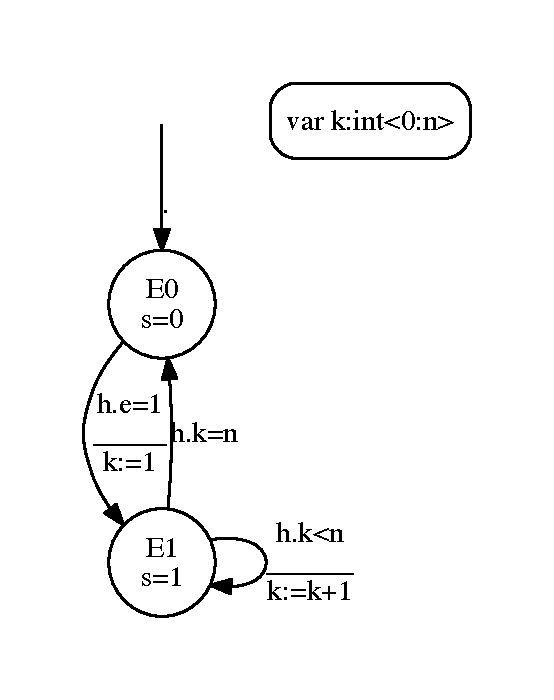
\includegraphics[width=0.25\linewidth]{figs/gensig-model}
\end{tabular}

\newpage
\subsection*{Rules}
\label{sec:static-rules}

\newcommand{\senv}[1]{\Gamma_{\!\mathsf{#1}}}

\step Rule \textsc{Program} gives the static interpretation of a program. The static environment
$\senv{M}$ (resp. $\senv{I}$) records the (typed) declarations of models (resp. IOs). 

\infrule[Program]
{\ut{fsm\_model}^+ \xrightarrow{} \senv{M} \\
 \ut{io\_decl}^+ \xrightarrow{} \senv{I} \\
 \senv{M},\senv{I} \vdash\ \ut{fsm_inst}^+ \xrightarrow{} M \\
 C=\mathcal{L}(\senv{I})}
{\tm{program}~\ut{fsm\_model}^+~\ut{io\_decl}^+~\ut{fsm\_inst}^+ \xrightarrow{} M, C}

The $\mathcal{L}$ function builds a static context $C$ from the IO environment $\senv{I}$~:
\begin{eqnarray*}
\mathcal{L}(\senv{I}) = \ttttttuple{I_e}{I_v}{O_e}{O_v}{H_e}{H_v}
\end{eqnarray*}
\noindent
where
\begin{eqnarray*}
I_e=\{x \in \text{dom}(\senv{I}) ~|~ \senv{I}(x)=\ttuple{\cat{input}}{\tm{event}}\} &
I_v=\{x \in \text{dom}(\senv{I}) ~|~ \senv{I}(x)=\ttuple{\cat{input}}{\tau},\ \tau\not=\tm{event}\}\\
O_e=\{x \in \text{dom}(\senv{I}) ~|~ \senv{I}(x)=\ttuple{\cat{output}}{\tm{event}}\} &
O_v=\{x \in \text{dom}(\senv{I}) ~|~ \senv{I}(x)=\ttuple{\cat{output}}{\tau},\ \tau\not=\tm{event}\}\\
H_e=\{x \in \text{dom}(\senv{I}) ~|~ \senv{I}(x)=\ttuple{\cat{shared}}{\tm{event}}\} &
H_v=\{x \in \text{dom}(\senv{I}) ~|~ \senv{I}(x)=\ttuple{\cat{shared}}{\tau},\ \tau\not=\tm{event}\}
\end{eqnarray*}

\medskip\step
Rule \textsc{Models} gives the interpretation of model declarations, giving an environment
$\senv{M}$. 

\infrule[Models]
{\falln{i}{1}{n}\quad \senv{M}^{i-1},\ \ut{fsm\_model}_i \xrightarrow{} \senv{M}^i \\
  \senv{M}^0 = \emptyset\quad
  \senv{M} = \senv{M}^n}
{\squn{\ut{fsm\_model}} \xrightarrow{} \senv{M}}

\medskip\step
Rule \textsc{Model} gives the interpretation of a single model declaration. It just records the
corresponding description in the environment $\senv{M}$, after performing some sanity checks, using
the $\mathsf{valid\_model}$ function, not detailed here. This function checks that~:
\begin{itemize}
\item all variable names occuring in guards are listed as input or local variable,
\item all expressions occuring in the guards of a transition have type $\mathsf{bool}$,
\item \ldots \todo{TBC}
\end{itemize}

\infrule[Model]
{\mm=\ttttttuple{Q}{I}{O}{V}{T}{\tau_0}\quad
  \mathsf{valid\_model}(\mm)}
{\tm{fsm\ model}~\cat{id}~I~O~Q~V~T~\tau_0 \xrightarrow{} \senv{M}[\cat{id}\mapsto\mm]}

\medskip\step
Rules \textsc{IOs} and \textsc{IO} give the interpretation of IO declarations, producing an environment
$\senv{I}$ binding names to a pair $\ttuple{\ut{io\_cat}}{\ut{typ}}$.

\infrule[IOs]
{\falln{i}{1}{n}\quad \senv{I}^{i-1},\ \ut{io_decl}_i \xrightarrow{} \senv{I}^i \\
 \senv{I}^0 = \emptyset\quad
  \senv{I} = \senv{I}^n}
{\squn{\ut{io\_decl}} \xrightarrow{} \senv{I}}

\infrule[IO]
{}
{\senv{I},\ \ut{cat}~\tm{id}~\tm{:}~\ut{typ} \xrightarrow{} \senv{I}[\tm{id}\mapsto
  \ttuple{\ut{cat}}{\ut{typ}}]}

\medskip\step
Rules \textsc{Insts} gives the interpretation of FSM instance declarations.

\infrule[Insts]
{\falln{i}{1}{n}\quad \senv{M},\senv{I} \vdash\ \ut{fsm\_inst}_i \xrightarrow{} \mu_i\\
  M=\sequn{\mu}}
{\squn{\ut{fsm\_inst}} \xrightarrow{} \mathcal{H}=\ttuple{M}{C}}

\step Rule \textsc{Inst} gives the interpretation of a single FSM instance as an automaton.

\newcommand{\tysequm}[3]{\langle#1_1\tm{:}#2_1,\ldots;#1_#3\tm{:}#2_#3\rangle}

\infrule[Inst]
{\senv{M}(\cat{id}) = \ttttttuple{\tysequm{i'}{\tau'}{m}}{\tysequm{o'}{\tau''}{n}}{Q}{V}{T}{\ttuple{q_0}{\vec{a_0}}}\\
  \Phi=\{i'_1 \mapsto i_1, \ldots, i'_m \mapsto i_m, o'_1 \mapsto o_1, \ldots, \o'_n \mapsto o_n \}\\
  \falln{i}{1}{m}\, \senv{I}(i_i)=\ttuple{\cat{cat}_i}{\tau_i},\ \cat{cat}_i \in
  \{\tm{input},\tm{shared}\} \wedge \tau_i=\tau'_i\\
  \falln{i}{1}{n}\, \senv{I}(o_i)=\ttuple{\cat{cat}_i}{\tau_i},\ \cat{cat}_i \in
  \{\tm{output},\tm{shared}\} \wedge \tau_i=\tau''_i\\
 \mm'=\ttttttuple{\tysequm{i}{\tau'}{m}}{\tysequm{o}{\tau''}{n}}{Q}{V}{\Phi_T(T)}{\ttuple{q_0}{\Phi_A(\vec{a_0})}}\\
 \mu=\tttuple{\mm'}{q_0}{\mathcal{I}(V)}}
{\senv{M},\senv{I} \vdash\ \tm{fsm}~\cat{id}~\sequm{i}{m}~\sequm{o}{n} \xrightarrow{} \mu}

Rule \textsc{Inst} checks the arity and the type conformance of the inputs and outputs supplied to
the instanciated model. The rule builds a \emph{substitution} $\Phi$ for binding \emph{local} input and
output names to \emph{global} ones. This substitution is applied to each transition (including the
initial one) of the resulting automaton~ using the derived functions $\Phi_T$ and $\Phi_A$ (not
detailed here).
% \begin{eqnarray*}
%  \Phi_T(\{\tau_1,\ldots,\tau_n\}) & = & \{ \Phi_\tau(\tau_1), \ldots, \Phi_\tau(\tau_n) \}\\
%  \Phi_\tau(\ttttuple{q}{\ttuple{e}{\{exp_1,\ldots,exp_m\}}}{\sequn{a}}{q'}) & = & 
% \ttttuple{q}{\ttuple{\Phi(e)}{\{\Phi_E(exp_1),\ldots,\Phi_E(exp_m)\}}}{\sequn{\Phi_A(a)}}{q'})
% \end{eqnarray*}
The $\mathcal{I}$ function builds an environment from a set of names, initializing each
  binding with the $\bot$ (``undefined'') value~:
  $$
  \mathcal{I}(\setn{x}) = \{x_1 \mapsto \bot, \ldots, x_n \mapsto \bot \}
  $$

\section{Dynamic semantic}
\label{sec:dynamic-semantics}

The dynamic semantics of a \textsc{Core Rfsm} program will be given in terms of (instantaneous)
\textbf{reactions}.
% TO BE INSERTED LATER ?
% It is similar to that of so-called \emph{synchronous languages} like
% \textsc{Esterel} or \textsc{Lustre}. Each reaction takes place at a given \emph{instant}. An instant
% is defined by the occurrence of an event (or of several simultaneous events). There's no reference
% to a notion of duration and time is only defined by the succession of instants (and hence of
% events). At each instant, each FSM composing the program takes at most one transition. 

\begin{eqnarray*}
  \mathcal{C} \vdash\ M,\ \env \xrightarrow[\rho]{\sigma} M',\ \env' 
\end{eqnarray*}

meaning

\begin{center}
``in the static context $\mathcal{C}$ and given a (dynamic) environment $\Gamma$, a set of
automata $M$ reacts to a \emph{stimulus} $\sigma$ leading to an updated set of automata $M'$, an
updated environment $\Gamma'$ and producing a \emph{response} $\rho$''
\end{center}

\subsection*{Definitions}
\label{sec:dynsem-defs}

\step Given an expression $\expr$ and an environment $\env$, $\eval{\env}{\expr}$ denotes the value obtained by
\textbf{evaluating} expression $\expr$ within environment $\env$. For example

$$
\eval{\{x\mapsto 1,y\mapsto 2\}}{x+y} = 3
$$

\medskip \step An \textbf{event} $e$ is either the occurrence of a \emph{pure event}
$\epsilon$ or the assignation of a \textbf{value} \emph{v} to a \textbf{name} (input, output or
local variable)~:

\begin{equation*}
  e = \begin{cases}
             \epsilon \\
             x \gets v
             \end{cases}
\end{equation*}

\medskip
\step An \textbf{event set} $E$ is a dated set of events

\begin{eqnarray*}
  E = \ttuple{t}{\setn{e}}
\end{eqnarray*}

where $t$ gives the occurrence \textbf{time} (logical instant).

\medskip
For example $E=\ttuple{10}{\{h,e \gets 0\}}$ means

\begin{center}
``At time t=10, event \texttt{h} occurs and (input) $e$ is set to 0'' .
\end{center}

\medskip
The union of \emph{event sets} is defined as
  \begin{eqnarray*}
    \ttuple{t}{e} \cup \ttuple{t'}{e'} =
    \begin{cases}
      \ttuple{t}{e \cup e'} \qquad \text{if}\ t=t' \\
      \bot\qquad \text{otherwise}
    \end{cases}
  \end{eqnarray*}

\medskip\step A \textbf{stimulus} $\sigma$ (resp. \textbf{response} $\rho$) is just an event set involving inputs
  (resp. outputs).
\todo{Input et output par rapport à quoi : automate ou contexte ?}

% \medskip
% \step A \textbf{program} $M$ is a set of automata

% \begin{equation*}
%   M = \setn{\mu}
% \end{equation*}

\subsection*{Rules}
\label{sec:dynsem-rules}

\step
Given a static description $\mathcal{H}=\ttuple{M}{C}$ of a program, the \textbf{execution} of this
program submitted to a sequence of stimuli $\vec{\sigma}=\sigma_1,\ldots,\sigma_n$ is formalized by
rule \textsc{Exec} 

% Rule \textsc{Exec} formalizes the execution of a program the reaction of a set of automata $M$
% in response to a sequence of stimuli $\sigma_1,\ldots,\sigma_n$

\infrule[Exec]
{  C \vdash\ M \xrightarrow{} M_0,\ \env_0\\
  \falln{i}{1}{n}\quad C \vdash\ M_{i-1},\ \env_{i-1} \xrightarrow[\rho_i]{\sigma_i} M_i,\ \env_i}
{\mathcal{H}=\ttuple{M}{C} \xrightarrow[\vec{\rho}=\sequn{\rho}]{\vec{\sigma}=\sequn{\sigma}} M_n,\ \env_n}

In other words, the execution of the program is described as as a sequence of \textbf{instantaneous
reactions}, which can be denoted as\footnote{Omitting context $C$, which is constant during an
execution.}~:

\begin{eqnarray*}
  M_0,\ \env_0 \xrightarrow[\rho_1]{\sigma_1} M_1,\ \env_1 \rightarrow \ldots
  \xrightarrow[\rho_n]{\sigma_n} M_n,\ \env_n
\end{eqnarray*}

\noindent where
\begin{itemize}
\item the \emph{global environment} $\Gamma$ here records the value of inputs and shared
  variables\footnote{This environment is required to handle events describing modifications of these
    values, as described below (see rule \textsc{ReactUpd}).},
\item $\rho_1, \ldots, \rho_n$ is the sequence of responses,
  \item $M_n$ and $\Gamma_n$ respectively give the final state of the automata and global
    environment.
\end{itemize}
  
\medskip \step
Rule \textsc{Init} describes how the initial set of automata $M_0$ and global environment
$\env_0$ are initialized by executing the initial transition of each automaton (producing a set of
initial responses $\rho_0$. 

\infrule[Init]
{\falln{i}{1}{n} \mu_i=\tttuple{\mm_i}{q_i}{\vars_i}\quad
  \mm_i=\ttttttuple{.}{.}{.}{.}{.}{\ttuple{.}{\vec{a_i}}}\quad
  C \vdash\ \vars_i,\ \gamma_{i-1} \xrightarrow[\ttuple{0}{\emptyset}]{\vec{a_i},0} \vars'_i,\ \gamma_i\quad
  \mu'_i=\tttuple{\mm_i}{q_i}{\vars'_i}\\
  C=\ttttttuple{.}{I_v}{.}{O_v}{.}{H_v}\quad
  \gamma_0 = \mathcal{I}(I_v \cup O_v \cup H_v)}
{C \vdash\ M=\setn{\mu} \xrightarrow{} M_0=\setn{\mu'},\ \env_0=\gamma_n}


\noindent
where the $I_v$, $O_v$ and $H_v$ sets, taken from the static context $C$, respectively give the name of
  inputs, outputs and shared variables.

\medskip
\textbf{Note}. Rule \textsc{Init} does \emph{not} produce any response
$\rho$. This is because the initial actions of an automaton cannot emit events hence can only update the
its local environment or the global one.

\medskip \step Rule \textsc{Acts} describes how a sequence of actions $\vec{a}$ (at time
$t$) updates the local and global environments, possibly emitting a set of responses\footnote{This
  set of responses is always empty when rule \textsc{Acts} is invoked in the context of \textsc{Init}.}.

\infrule[Acts]
{ \falln{i}{1}{n}\quad C \vdash\ \vars_{i-1},\ \env_{i-1} \xrightarrow[\rho_i]{a_i,\ t} \vars_i,\ \env_i\\
  \vars_0=\vars\quad \env_0=\env \quad \rho_e = \cuppn{\rho_i}}
{C \vdash\ \vars,\ \env \xrightarrow[\rho_e]{\sequn{a},\ t} \vars_n,\ \env_n}

\medskip \textbf{Note}. The definition of rule \textsc{Acts} given above enforces a \emph{sequential
  interpretation} of actions. For example
$$
\{x \mapsto 1,\ s \mapsto \bot \},\ \env \xrightarrow{\ssequ{x \gets x+1}{s \gets x},t}
\{x \mapsto 2,\ s \mapsto 2 \}, \env
$$
Rule \textsc{Acts} could easily be reformulated to describe other interpretations, such as a
\emph{synchronous} one, in which all RHS values are first evaluated
and then assigned to LHS in parallel\footnote{As happens in hardware synchronous implementations for
  example.}.
% for example~:
% $$
% \{x \mapsto 1,\ s \mapsto \bot \},\ \env \xrightarrow{\ttuple{\vec{a}}{d}}_A
% \{x \mapsto 2,\ s \mapsto 1 \}, \env
% $$


\medskip \step Rules \textsc{ActUpdL} and \textsc{ActUpdG} respectively describe the
effect of an action updating a local or global variable (shared variable or output)\footnote{The
  effect of an action emitting an event will be described by rules \textsc{ActEmitS} and \textsc{ActEmitG},
  given latter.}.

\begin{multicols}{2}
\infrule[ActUpdL]
{x \in \text{dom}(\vars) \quad v = \eval{\vars\cup\env}{\expr}}
{C \vdash\ \vars,\ \env \xrightarrow[\ttuple{t}{\emptyset}]{x\gets \expr,\ t} \vars[x\mapsto v],\ \env}

\infrule[ActUpdG]
{x \in \text{dom}(\env) \quad v = \eval{\vars\cup\env}{\expr}}
{C \vdash\ \vars,\ \env \xrightarrow[\ttuple{t}{\emptyset}]{x\gets \expr,\ t} \vars,\ \env[x\mapsto v]}
\end{multicols}

\step Rule \textsc{React} describes how a program $M$ within a global environment $\env$
(instantaneously) reacts to a stimulus (event set) $\sigma$, producing a response (event set)
$\rho$, an updated program $M'$ and an updated environment $\env'$.

\infrule[React]
{\sigma_e,\sigma_v = \Sigma(\sigma)\qquad
 C \vdash\ M,\ \env \xrightarrow{\sigma_v} M,\ \env_v\qquad
 C \vdash\ M,\ \env_v \xrightarrow[\rho_e]{\sigma_e} M',\ \env'}
{C \vdash\ M,\ \env \xrightarrow[\rho_e]{\sigma} M',\ \env'}

where the function $\Sigma$ partitions a \emph{event set} into one containing the stimuli
corresponding to \emph{pure} events ($\epsilon$) and another containing those corresponding to updates to
global inputs~:

\begin{equation*}
  \Sigma(\ttuple{t}{\setn{e}}) = \ttuple{t}{\{ e_i ~|~ e_i = \epsilon_i \}},\quad\ttuple{t}{\{
        e_i ~|~ e_i = x_i \gets v_i \}}
\end{equation*}

\step Rule \textsc{ReactUpd} describes how a program $M$ within a global environment $\env$ reacts to set
of events describing updates to global inputs. These updates are just recorded in the environment and do not produce
responses, nor trigger any reaction of the automata~:

\infrule[ReactUpd]
{}
{C \vdash\ M,\ \env \xrightarrow{\sigma_v=\ttuple{t}{\{x_1\gets v_1,\ldots,x_m\gets v_m\}}} M,\ \env[x_1\mapsto
  v_1]\ldots[x_m\mapsto v_m]}

\step
Rule \textsc{ReactEv} describes how a program reacts to a set of pure events.

\infrule[ReactEv]
{\falln{i}{1}{n} C \vdash\ \mu_{\pi(i)},\ \env_{i-1} \xrightarrow[\rho_i]{\sigma_i} \mu'_{\pi(i)},\ \env_i\qquad
 \sigma_i=\sigma_{i-1} \cup \rho_i\\
 \env_0 = \env\qquad 
 \sigma_0 = \sigma_e\qquad
 \rho_e = \cuppn{\rho_i}\qquad
 \env'=\env_n}
{C \vdash\ M=\setn{\mu}, \env \xrightarrow[\rho]{\sigma_e=\ttuple{t}{\{\epsilon_1,\ldots,\epsilon_m\}}}_e
  M'=\setn{\mu'},\ \env'}

Each automaton reacts
separately but \emph{in a specific order}. This order is derived from the dependencies between
automata. We say that an automaton $\mu'$ \emph{depends on} another automaton $\mu$ at a given
instant $t$, and note

\begin{eqnarray*}
  \mu \leq \mu'
\end{eqnarray*}

if the reaction of $\mu$ at this instant can trigger or modify the reaction of $\mu'$
at the same instant. Concretely, this happens when $\mu$ and $\mu'$ are respectively in states $q$
and $q'$ and there's (at least) one pair of transitions $(\tau,\tau')$ starting respectively from
$q$ and $q'$ so that
\begin{itemize}
\item $\tau'$ is triggered by an event emitted by $\tau$, or
\item a variable occuring in the guards associated to $\tau'$ is written by the actions associated
  to $\tau$.
\end{itemize}

The function $\pi$ used in \textsc{ReactEv} is a permutation of $\{1,\ldots,n\}$ defined so that
\begin{eqnarray*}
  \mu_{\pi(1)} \leq \mu_{\pi(2)} \leq \ldots \leq \mu_{\pi(n)}
\end{eqnarray*}

Having the automata of $M$ react in the order $\pi(1),\ldots,\pi(n)$ ensures that any event emitted or local
variable update performed by an automaton during a given reaction is effectively perceived by any
other automaton \emph{at the same reaction}, a principle called \emph{instantaneous broadcats}.

The permutation $\pi$ can easily be computed by a \emph{topological sort} of the dependency graph
derived from the conditions expressed above. In practice, this will be carried out by a static
analysis of the program. 

\step Rules \textsc{React1}, \textsc{React0} and \textsc{ReactN} describe how a single automaton reacts to a
set of pure events, updating both its internal and global states and producing another set of (pure)
events in response.

\begin{multicols}{2}
\infrule[React1]
{ \Delta_{\env \cup \vars}(\mm,q,e) = \{ \tau \}\\
  C \vdash\ \mu,\ \env \xrightarrow[\rho_e]{\tau,\ t} \mu', \env'}
{C \vdash\ \mu=\tttuple{\mm}{q}{\vars},\ \env \xrightarrow[\rho_e]{\sigma_e=\ttuple{t}{e}} \mu',\ \env'}

\infrule[React0]
{ \Delta_{\env \cup \vars}(\mm,q,e) = \emptyset}
{C \vdash\ \mu=\tttuple{\mm}{q}{\vars},\ \env \xrightarrow[\ttuple{t}{\emptyset}]{\sigma_e=\ttuple{t}{e}} \mu,\ \env}
\end{multicols}

\infrule[ReactN]
{ \Delta_{\env \cup \vars}(\mm,q,e) = \setn{\tau}\\
  \tau = \mathsf{choice}(\setn{\tau})\\
  C \vdash\ \mu,\ \env \xrightarrow[\rho_e]{\tau,\ t} \mu', \env'}
{C \vdash\ \mu=\tttuple{\mm}{q}{\vars},\ \env \xrightarrow[\rho_e]{\sigma_e=\ttuple{t}{e}} \mu',\ \env'}

Given a automaton modelised by $\mm$ and currently in state $q$, $\Delta_\env(\mm,q,e)$, where
$e=\setn{\epsilon}$, returns
the set of \emph{fireable} transitions, \emph{i.e.} all the transitions triggered by the event set
$e$ starting from $q$ and for which the all the associated boolean guards evaluate, in environment $\env$, to
\textsf{true}.

\begin{equation*}
  \Delta_\env(\mathcal{M},q,\setn{\epsilon}) = \cupp{i=1}{n}{\Delta_\env(\mathcal{M},q,\epsilon_i)}
\end{equation*}
where
\begin{equation*}
 \Delta_\env(\ttttttuple{.}{.}{.}{.}{T}{.},q,\epsilon) = \{ (q_s,c,a,q_d) \in T ~|~
  q=q_s ~\wedge~ c = \ttuple{\epsilon}{\setn{e}} ~\wedge~ \falln{i}{1}{n} \eval{\env}{e_i} = \mathsf{true} \}
\end{equation*}


Rule \textsc{React1} describes the case when the set of events triggers exactly \emph{one} transition
of the automaton. Its state and local variables are updated according to the actions listed in the
transition and the remaining actions are used to generated the set of responses.

Rule \textsc{React0} describes the case when the set of events does not trigger any transition. The
automaton and the global environment are left unchanged.

Rule \textsc{ReactN} describes the case when the set of events triggers more than one transition. This
situation corresponds to a non-deterministic behavior of the automaton. The
function \textsf{choice} is here used to choose one transition\footnote{This can done, for example,
  by adding a \emph{priority} to each transition.}. 

\medskip \step
Rule \textsc{Trans} describes the effect of performing a transition, updating the automaton local
and global states and returning a set of (pure) events as responses.

\infrule[Trans]
{\mu=\tttuple{\mm}{q}{\vars} \qquad \tau=\ttttuple{q}{c}{\vec{a}}{q'} \\
  C \vdash\ \vars,\ \env \xrightarrow[\rho_e]{\vec{a},t}_a \vars',\ \env'\\
  \mu'=\tttuple{\mm}{q'}{\vars'}}
{C \vdash\ \mu,\ \env \xrightarrow[\rho_e]{\tau,\ t} \mu',\ \env'}

\medskip\step Rules \textsc{ActEmitS} and \textsc{ActEmitG} complement the rules \textsc{ActUpdL} and \textsc{ActUpdG}
given previously by describing the effect of an action emitting a shared or output event. The
$H_e$ set, taken from context $C$, is here used to distinguish between to to. The formers can trigger the reaction of other(s)
automaton(s), the latters are just ignored here (see note below).

\begin{multicols}{2}
\infrule[ActEmitS]
{C=\ttttttuple{.}{.}{.}{.}{H_e}{.}\quad
  \epsilon \in H_e} 
{C \vdash\ \vars,\ \env \xrightarrow[\ttuple{t}{\{\epsilon\}}]{\epsilon,\ t} \vars,\ \env}

\infrule[ActEmitG]
{C=\ttttttuple{.}{.}{.}{.}{H_e}{.}\quad
 \epsilon \not\in H_e} 
{C \vdash\ \vars,\ \env \xrightarrow[\ttuple{t}{\emptyset}]{\epsilon,\ t} \vars,\ \env}
\end{multicols}

\bigskip
\textbf{Note}.
The semantics described here only defines how a program execution progresses, from the initial
program to the final program state $M$. In practice, an interpreter will also build a \emph{trace}
of such an execution, recording all significant events (stimuli, responses, state moves,
\emph{etc.}). Building such a trace is easily performed by modifying the semantic rules given above. It
has not been done here for the sake of simplicity.

%%% Local Variables:
%%% mode: latex
%%% TeX-master: "rfsm"
%%% End:
   
\chapter*{Appendix B - Compiler options}
\label{cha:compiler-options}

Compiler usage : \verb|rfsmc [options...] files|

\medskip
\begin{tabular}[c]{ll}
-lib & set location of the support library (default: /usr/local/rfsm/lib)\\
-dump\_model & dump model in text format to stdout\\
-target\_dir & set target directory (default: .)\\
-dot & generate top-level .dot representation(s)\\
-sim & run simulation (generating .vcd file)\\
-ctask & generate CTask code\\
-systemc & generate SystemC code\\
-vhdl & generate VHDL code\\
-version & print version of the compiler and quit\\
-dot\_no\_captions & Remove captions in .dot representation(s)\\
-dot\_fsm\_insts & generate .dot representation of all FSM instances\\
-dot\_fsm\_models & generate .dot representation of all FSM models\\
-dot\_actions\_nl & write actions with with a separating newline\\
-trace & set trace level for simulation (default: 0)\\
-vcd & set name of .vcd output file when running simulation (default: run.vcd)\\
-synchronous\_actions & interpret actions synchronously\\
-sc\_time\_unit & set time unit for the SystemC test-bench (default: SC\_NS)\\
-sc\_trace & set trace mode for SystemC backend (default: false)\\
-stop\_time & set stop time for the SystemC and VHDL test-bench (default: 100)\\
-sc\_double\_float & implement float type as C++ double instead of float (default: false)\\
-vhdl\_trace & set trace mode for VHDL backend (default: false)\\
-vhdl\_time\_unit & set time unit for the VHDL test-bench\\
-vhdl\_ev\_duration & set duration of event signals (default: 1 ns)\\
-vhdl\_rst\_duration & set duration of reset signals (default: 1 ns)\\
-vhdl\_numeric\_std & translate integers as numeric\_std [un]signed (default: false)\\
-vhdl\_bool\_as\_bool & translate all booleans as boolean (default: false)\\

\end{tabular}

\normalsize

%%% Local Variables: 
%%% mode: latex
%%% TeX-master: "rfsm"
%%% End: 

\chapter{ Building language variants}
\label{cha:variants}

Following the approach described in~\cite{Leroy00} for example, the RFSM compiler is implemented in
a \emph{modular} way. The language is split into a \emph{host} language, describing the general
structure and behavior of FSMs (states, transitions, \ldots) and a \emph{guest}
language\footnote{``Base'' in the terminology of \cite{Leroy00}.} describing the syntax and
semantics of \emph{expressions} used in transition guards and semantics. 
Technically, this ``separation of concern'' is realized by providing the host language in the form
of a \emph{functor} taking as argument the module implementing the guest language.

This approach makes it fairly easy to produce variants of the ``standard'' RFSM language -- with
dedicated type systems and expression languages typically -- by simply defining the module defining
the guest language and applying the aforementioned functor. Actually, the full, ``standard'', RFSM
  language was designed using this approach, starting from a very simple ``core'' guest
  language gradually enriched with new features at the expression level\footnote{Traces of the
    incremental design process can be found in the \texttt{srs/guests/core},
    \texttt{src/guests/others/szdints} and \texttt{src/guests/others/szvars} directories for example.}. 

The directory \verb|src/guests/templ| in the distribution provides the basic structure for deploying
this approach. In practice, to implement a language variant, one has to
\begin{itemize}
\item write the implementation of the guest language in the form of a collection of modules in the
  \texttt{lib} subdirectory\footnote{These modules will be encapsulated in a single module and the
    latter will be passed to the host functor to build the target language.},
\item write the lexer and the parser for this guest language (expressions, type expressions, \ldots),
\item build the compiler by simply invoking \emph{make}  
\end{itemize}

\medskip
To illustrate this process, we describe in the sequel the implementation of a very simple language
language for which the guest language has only two types, `event` and `bool`,
and expressions are limited to boolean constants and variables\footnote{This language is essentially
  that provided in \texttt{src/guests/others/mini}.}. We focus here on the most salient features. 
The \texttt{Readme} file in the  \texttt{templ} directory describes the procedure in
details. Other examples, given in \verb|src/guests/core| and \verb|src/guests/others|\footnote{And, of
  course, in \texttt{src/guests/full}.}, can also be used as guidelines. 

\section{Implementing the \texttt{Guest} module}

The module implementing the guest language must match the following signature~:

\begin{lstlisting}[language={[Objective]Caml},frame=single,basicstyle=\small,label={lst:guest-sig}]
module type T = sig
  module Info : INFO
  module Types : TYPES
  module Syntax : SYNTAX with module Types = Types
  module Typing : TYPING with module Syntax = Syntax and module Types = Types
  module Value : VALUE with type typ = Types.typ
  module Static : STATIC with type expr = Syntax.expr and type value = Value.t
  module Eval : EVAL with module Syntax = Syntax and module Value = Value
  module Ctask: CTASK with module Syntax = Syntax
  module Systemc: SYSTEMC with module Syntax = Syntax and module Static = Static and type value = Value.t
  module Vhdl: VHDL with module Syntax = Syntax and module Static = Static and type value = Value.t
  module Error : ERROR
  module Options : OPTIONS
end
\end{lstlisting}

\noindent
where
\begin{itemize}
\item module \texttt{Info} gives the name and version of the guest language,
\item module \texttt{Syntax} describes the (abstract) syntax of the guest language,
\item modules \texttt{Types} and \texttt{Typing} respectively describe the types and the typing
  rules of the guest language,
\item module \texttt{Static} describes the static semantics of the guest language (basically, the
  interpretation of model parameters),
\item modules \texttt{Value} and \texttt{Eval} respectively describe the values and the dynamic
  semantics manipulating these values,
\item modules \texttt{CTask}, \texttt{Systemc} and \texttt{Vhdl} respectively describe the
  guest-level part of the C, SystemC and VHDL backends,
\item module \texttt{Error} describes how guest-specific errors are handled,
\item module \texttt{Options} describes guest-specific compiler options.
\end{itemize}

Listings~\ref{lst:mini-types}, \ref{lst:mini-syntax},\ref{lst:mini-value} and \ref{lst:mini-eval}
respectively show the contents of of the \texttt{Types},
\texttt{Syntax}, \texttt{Value} and \texttt{Eval} modules for the \texttt{mini} language.
The definition of non essential fonctions has been omitted\footnote{See the corresponding source files in
  \texttt{src/guests/others/mini/lib} for a complete listing.}.

\begin{lstlisting}[language={[Objective]Caml},frame=single,basicstyle=\small,caption={Module
    \texttt{Guest.Types} (excerpt)},label={lst:mini-types}]
type typ =
  | TyEvent
  | TyBool
  | TyUnknown

let no_type =  TyUnknown

let is_event_type (t: typ) = match t with TyEvent -> true | _ -> false
let is_bool_type (t: typ) =  match t with TyBool -> true | _ -> false

let pp_typ ?(abbrev=false) fmt (t: typ) = ...
\end{lstlisting}

In module \texttt{Types}, the key definition is that of type \texttt{typ}, which describes the
guest-level types, \emph{i.e.} the types which can be attributed to guest-level expressions and
variables. The type \texttt{TyUnknown} is used to define the value \texttt{no_type} which is
attributed by the host language to (yet) untyped syntax elements.

\begin{lstlisting}[language={[Objective]Caml},frame=single,basicstyle=\small,caption={Module
    \texttt{Guest.Syntax} (excerpt)}, label={lst:mini-syntax}]
module Types = Types

module Location = Rfsm.Location
module Annot = Rfsm.Annot
module Ident = Rfsm.Ident

let mk ~loc x = Annot.mk ~loc ~typ:Types.no_type x

(* Type expressions *)

type type_expr = (type_expr_desc,Types.typ) Annot.t
and type_expr_desc = TeConstr of string (* name, no args here *)

let is_bool_type (te: type_expr) = ...
let is_event_type (te: type_expr) = ...

let pp_type_expr fmt (te: type_expr) =  ...

(* Expressions *)
  
type expr = (expr_desc,Types.typ) Annot.t
and expr_desc = 
  | EVar of Ident.t
  | EBool of bool

let vars_of_expr (e: expr) = ...
and pp_expr fmt (e: expr) = ...

(* LHSs *)
  
type lhs = (lhs_desc,Types.typ) Annot.t
and lhs_desc = Ident.t

let lhs_var (l: lhs) = ...
let vars_of_lhs (l: lhs) = ...
let is_simple_lhs (l: lhs) = true

let mk_simple_lhs (v: Ident.t) =
  Annot.{ desc=v; typ=Types.no_type; loc=Location.no_location }

let pp_lhs fmt l =  ...
\end{lstlisting}

The module \texttt{Syntax} use the modules \texttt{Location}, \texttt{Annot}  and \texttt{Ident}
provided by the \texttt{Rfsm} host library. These modules provide types and functions to handle
source code locations, syntax annotations and identifiers respectively. The type
\verb|('a,Types.typ) Annot.t| is associated to syntax nodes of type
\verb|'a|. The types \verb|type_expr|, \verb|expr| and \verb|lhs| respectively describe guest-level
type expressions, expressions and left-hand-sides (LHS). LHS are used in the definition of
actions. In this language they are limited to simple identifiers (ex: \verb|x:=<expr>|) but the
guest language can use other forms (like in the RFSM ``full'' language which support arrays and
records in LHS). 

\begin{lstlisting}[language={[Objective]Caml},frame=single,basicstyle=\small,caption={Module
    \texttt{Guest.Values} (excerpt)},label={lst:mini-value}]
type typ =
  | TyEvent
  | TyBool
  | TyUnknown

let no_type =  TyUnknown

let is_event_type t = match t with TyEvent -> true | _ -> false
let is_bool_type t =  match t with TyBool -> true | _ -> false
let mk_type_fun ty_args ty_res = ...

let pp_typ ?(abbrev=false) fmt t = ...
\end{lstlisting}

\begin{lstlisting}[language={[Objective]Caml},frame=single,basicstyle=\small,caption={Module
    \texttt{Guest.Value} (excerpt)},label={lst:mini-value}]
type t =
  | Val_bool of bool
  | Val_unknown

let default_value ty = match ty with
  | _ -> Val_unknown

exception Unsupported_vcd of t

let vcd_type (v: t) = match v with
  | Val_bool _ -> Rfsm.Vcd_types.TyBool
  | _ -> raise (Unsupported_vcd v)

let vcd_value (v: t) = match v with
  | Val_bool v -> Rfsm.Vcd_types.Val_bool v
  | _ -> raise (Unsupported_vcd v)

let pp fmt (v: t) =  ...
\end{lstlisting}

The module \verb|Guest.Value| define the values, associated to guest-level expressions by the
dynamic semantics. The value \verb|Val_unknown| is used to represent undefined or unitialized
value. The functions \verb|vcd_type| and \verb|vcd_value| provide the interface to the VCD backend,
generating simulation traces~: they should return a VCD compatible representation  (defined in the
host library \verb|Vcd_types| module) of a value.

\begin{lstlisting}[language={[Objective]Caml},frame=single,basicstyle=\small,caption={Module
    \texttt{Guest.Eval} (excerpt)},label={lst:mini-eval}]
module Syntax = Syntax
module Value = Value
module Env = Rfsm.Env
module Annot = Rfsm.Annot

type env = Value.t Env.t

exception Illegal_expr of Syntax.expr
exception Uninitialized of Rfsm.Location.t

let mk_env () = Env.init []

let upd_env lhs v env = Env.upd lhs.Annot.desc v env

let lookup ~loc v env = 
 match Rfsm.Env.find v env with
  | Value.Val_unknown -> raise (Uninitialized loc)
  | v -> v

let eval_expr env e = match e.Annot.desc with
  | Syntax.EVar v -> lookup ~loc:e.Annot.loc v env
  | Syntax.EBool i -> Val_bool i 

let eval_bool env e = 
  match eval_expr env e with
  | Val_bool b -> b
  | _ -> raise (Illegal_expr e) 

let pp_env fmt env = ...
\end{lstlisting}

The module \verb|Guest.Eval| defines the guest-level dynamic semantics, \emph{i.e.} the definition
of the dynamic environment \texttt{env}, used to bind identifiers to values and of the 
functions \verb|eval_expr| and \verb|exal_bool| used to evaluate guest-level expressions. The
presence of a distinct, \verb|eval_bool| function is required because the boolean type and
expressions are not part of the host-level syntax. The definition of the \texttt{env} type here uses
that provided by the host library but any definition matching the corresponding signature would do.

\section{Implementing the \texttt{Guest} parser}

The parser for the guest language defines the concrete syntax for guest-level type expressions,
expressions and LHS. It is written in a separate \texttt{.mly} file which will be combined with the
parser for the host language\footnote{Using \texttt{menhir} facility to split parser specifications
  into multiple files.}. There are only two guest specific tokens here, denoting the boolean
constants \texttt{true} and \texttt{false}. The \texttt{open} directive in the prologue section
gives access to the abstract syntax definitions given in \texttt{Guest.Syntax} module. The function
\texttt{mk}, defined in this module, builds annotated syntax nodes, inserting the source code
location. 

\begin{lstlisting}[language={menhir},frame=single,basicstyle=\small,caption={File
    guest_parser.mly},label={lst:mini-eval}]
%token TRUE
%token FALSE

%{
open Mini.Top.Syntax
%}

%%
%public type_expr:
  | tc = LID { mk ~loc:$sloc (TeConstr tc) }

%public lhs:
  | v = LID { mk ~loc:$sloc (mk_ident v) }

%public expr:
  | v = LID { mk ~loc:$sloc (EVar (mk_ident v)) }
  | c = scalar_const { c }

%public scalar_const:
  | TRUE { mk ~loc:$sloc (EBool true) }
  | FALSE { mk ~loc:$sloc (EBool false) }

%public const:
  | c = scalar_const { c }

%public stim_const: 
  | c = scalar_const { c }

\end{lstlisting}

\section{Implementing the \texttt{Guest} lexer}

The \texttt{ocamllex} tool, used for defining the lexer, does not support multi-file definitions.
The lexer for the guest-specific part of the target language is therefore supplied in the form of
code fragments to be inserted in the host lexer definition file\footnote{Technically, this insertion is
  performed using the \texttt{cppo} tool.}. These fragments are listed in two separate files,
present in the \texttt{bin} subdirectory of the guest directory~:
\begin{itemize}
\item the file \texttt{guest_km} contains the lexer definition of the guest-specific keywords,
\item the file \texttt{guest_rules} contains the guest-specific rules.
\end{itemize}

In the case of the \texttt{mini} language defined here, the latter is empty and the former only
contains the two following lines.

\begin{verbatim}
"true", TRUE;
"false", FALSE;
\end{verbatim}

\section{Building the compiler}

Defining the target language implementation and building the associated compiler is then simply
obtained by the two following functor applications\footnote{For technical reasons, these two
  statements are placed in distinct files, \texttt{bin\/lang.ml} and \texttt{bin\/rfsmc.ml}.}~:

\begin{lstlisting}[language={[Objective]caml},frame=single,basicstyle=\small]
module L = Rfsm.Host.Make(Mini.Top)

module Compiler =
  Rfsm.Compiler.Make
    (L)
    (Lexer)
    (struct include Parser type program = L.Syntax.program end)
\end{lstlisting}

Invoking the compiler now boils down to executing

\begin{lstlisting}[language={[Objective]caml},frame=single,basicstyle=\small]
let _ = Printexc.print Compiler.main ()
\end{lstlisting}

%%% Local Variables:
%%% mode: latex
%%% TeX-master: "rfsm_rm"
%%% End:
   

% \input{source}
% \input{biblio}

\bibliographystyle{plain}
\bibliography{rfsm}

\end{document}

%%% Local Variables:
%%% mode: latex
%%% TeX-master: t
%%% End:
